\documentclass[aspectratio=169, 11pt]{beamer}

% =====================================================================
%  23CSE498 -- Project Phase 2 -- Panel Review 1
%  Automated Volleyball Tactical Analysis from Broadcast Video
%  Track: Application-Based Project
%
%  Deck kept deliberately minimal -- see DEFENSE_MASTER.md (repo root) for
%  the exhaustive prep material, Q&A answers, and every open item. Nothing
%  in that file belongs on a slide; it is for verbal answers only.
%
%  Compile: pdflatex panel_review_1.tex  (run twice for TikZ overlay + TOC)
%  No external files required. Optional: place logo.png beside this file.
% =====================================================================

\usepackage[utf8]{inputenc}
\usepackage[T1]{fontenc}
\usepackage{xcolor}
\usepackage{booktabs}
\usepackage{amsmath}
\usepackage{amssymb}
\usepackage{graphicx}
\usepackage{tikz}
\usetikzlibrary{calc, positioning, arrows.meta}

\graphicspath{{../}{./}}
\IfFileExists{opensans.sty}{\usepackage[default,scale=0.95]{opensans}}{}

\definecolor{amritaMaroon}{HTML}{A4123F}
\definecolor{okGreen}{HTML}{1B7A3D}

\usetheme{Madrid}
\usecolortheme[named=amritaMaroon]{structure}
\setbeamertemplate{navigation symbols}{}
\setbeamertemplate{footline}[frame number]
\setbeamertemplate{itemize items}[triangle]
\setbeamerfont{frametitle}{size=\large}
\setbeamerfont{framesubtitle}{size=\scriptsize}

\newcommand{\integ}{\textcolor{okGreen}{\textbf{\checkmark}}}
\newcommand{\R}{$\rightarrow$}

\setlength{\tabcolsep}{4pt}
\renewcommand{\arraystretch}{1.15}

\begin{document}

% =====================================================================
\begin{frame}
    \begin{tikzpicture}[remember picture,overlay]
        \node[fill=amritaMaroon, text=white, font=\bfseries\footnotesize, anchor=north east, rounded corners=2pt, inner sep=5pt]
        at ($(current page.north east) + (-0.2cm,-0.2cm)$) {Type 2: Application Project};
    \end{tikzpicture}
    \centering
    \IfFileExists{logo.png}{\includegraphics[width=2.6cm]{logo.png}\\[0.15cm]}{\vspace{1.1cm}}
    {\large \textbf{\textcolor{amritaMaroon}{Automated Volleyball Tactical Analysis\\ from Broadcast Video}}} \\
    \vspace{0.10cm}
    {\footnotesize Detection \R\ tracking \R\ court projection \R\ formation features \R\ tactical classification} \\
    \vspace{0.12cm}
    {\footnotesize \textbf{23CSE498 -- Project Phase 2 (Panel Review 1)} \quad | \quad \textbf{Team Number: [XX]}} \\
    \vspace{0.18cm}
    \begin{table}
        \centering \footnotesize \renewcommand{\arraystretch}{1.05}
        \begin{tabular}{|c|c|l|}
            \hline \textbf{S.No} & \textbf{Register Number} & \textbf{Student Name} \\ \hline
            1 & CB.EN.U4CSE23XXX & Student Name 1 \\ \hline
            2 & CB.EN.U4CSE23XXX & Student Name 2 \\ \hline
            3 & CB.EN.U4CSE23XXX & Student Name 3 \\ \hline
            4 & CB.EN.U4CSE23XXX & Student Name 4 \\ \hline
        \end{tabular}
    \end{table}
    {\footnotesize Guide: \textbf{Guide Name}, Designation, Department of CSE} \\
    \vspace{0.08cm}{\scriptsize \today}
\end{frame}

% =====================================================================
\begin{frame}{Outline}
    \small
    \begin{enumerate}
        \item \textbf{Application Architecture \& Workflow Design} \hfill (5 marks)
        \item \textbf{Implementation Progress ($\approx$60\%)} \hfill (8 marks)
        \item \textbf{Technical Knowledge \& Design Decisions} \hfill (5 marks)
        \item \textbf{Technical Enrichment}
    \end{enumerate}
\end{frame}

% #####################################################################
\section{Application Architecture \& Workflow Design}
% #####################################################################

\begin{frame}[t]{1.1\quad Problem, Users \& Requirements}
    \small
    \begin{columns}[t]
        \column{0.5\textwidth}
        \textbf{Problem.} Coaching staff need fast, objective feedback on
        \emph{whole-team spatial coordination}, not just individual actions
        or ball trajectory.

        \vspace{0.2cm}
        \textbf{Target users.} Volleyball coaches, performance analysts,
        sports-science researchers, from ordinary broadcast footage.

        \column{0.5\textwidth}
        \textbf{Functional requirements.}
        \begin{itemize}
            \item Ingest broadcast video, no manual court calibration.
            \item Classify $\approx$1\,s windows into 4 tactical classes.
            \item Emit CSV, annotated video, coordination report.
        \end{itemize}
        \vspace{0.15cm}
        \textbf{Non-functional requirements.}
        \begin{itemize}
            \item Commodity CPU at inference.
            \item Fail-loud: abort on degenerate input.
            \item One command regenerates every reported number.
        \end{itemize}
    \end{columns}
\end{frame}

\begin{frame}[t]{1.2\quad End-to-End System Architecture}
    \begin{center}
    \resizebox{\textwidth}{!}{%
    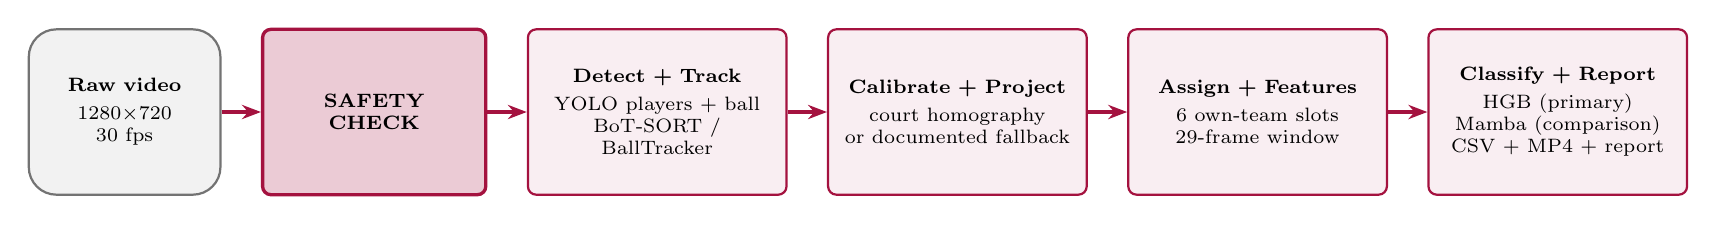
\begin{tikzpicture}[
        node distance=5mm,
        box/.style={draw=amritaMaroon, thick, fill=amritaMaroon!7, rounded corners=3pt,
                    text width=3.05cm, align=center, minimum height=2.1cm, font=\scriptsize},
        gate/.style={draw=amritaMaroon, very thick, fill=amritaMaroon!22, rounded corners=3pt,
                     text width=2.6cm, align=center, minimum height=2.1cm, font=\scriptsize\bfseries},
        io/.style={draw=black!55, thick, fill=black!5, rounded corners=10pt,
                   text width=2.2cm, align=center, minimum height=2.1cm, font=\scriptsize},
        fl/.style={-{Stealth[length=2.4mm]}, very thick, amritaMaroon}
    ]
        \node[io] (vid) {\textbf{Raw video}\\[2pt] 1280$\times$720\\ 30 fps};
        \node[gate, right=of vid] (gate) {SAFETY\\CHECK};
        \node[box, right=of gate] (perc) {\textbf{Detect + Track}\\[2pt] YOLO players + ball\\ BoT-SORT / BallTracker};
        \node[box, right=of perc] (proj) {\textbf{Calibrate + Project}\\[2pt] court homography\\ or documented fallback};
        \node[box, right=of proj] (feat) {\textbf{Assign + Features}\\[2pt] 6 own-team slots\\ 29-frame window};
        \node[box, right=of feat] (clf) {\textbf{Classify + Report}\\[2pt] HGB (primary)\\ Mamba (comparison)\\ CSV + MP4 + report};
        \draw[fl] (vid) -- (gate); \draw[fl] (gate) -- (perc); \draw[fl] (perc) -- (proj);
        \draw[fl] (proj) -- (feat); \draw[fl] (feat) -- (clf);
    \end{tikzpicture}}
    \end{center}
    \vspace{0.2cm}\footnotesize
    Both classifiers read the same $29\times18$ window: HGB as 132
    aggregated statistics, Mamba as the raw ordered sequence. The safety
    check aborts rather than emit a report on degenerate input.
\end{frame}

\begin{frame}[t]{1.3\quad Module Contract, Technology Stack \& Deployment}
    \scriptsize
    \begin{columns}[t]
        \column{0.58\textwidth}
        \begin{tabular}{@{}p{2.3cm}p{2.1cm}p{2.5cm}@{}}
            \toprule
            \textbf{Module} & \textbf{Consumes} & \textbf{Produces} \\
            \midrule
            Safety check     & video segment  & go / no-go \\
            Detect + track   & frame          & player/ball IDs \\
            Court calib.     & frame, boxes   & court coords \\
            Assign           & tracks, colour & 6 own-team players \\
            Features         & 29$\times$6 players & $Z \in \mathbb{R}^{29\times18}$ \\
            Classifier       & $Z$            & class + probs + confidence \\
            \bottomrule
        \end{tabular}
        \column{0.42\textwidth}
        \textbf{Stack:} Python, Ultralytics YOLO, OpenCV, ByteTrack/BoT-SORT,
        scikit-learn (HGB, primary), PyTorch (Mamba, comparison), pytest.

        \vspace{0.15cm}
        \textbf{Deployment:} CLI + batch runner; annotated MP4 + CSV output;
        \texttt{reproduce.py} regeneration harness.
    \end{columns}
\end{frame}

% #####################################################################
\section{Implementation Progress}
% #####################################################################

\begin{frame}[t]{2.1\quad Module Implementation Status ($\approx$60\%)}
    \scriptsize
    \begin{tabular}{@{}p{5.2cm}p{6.0cm}c@{}}
        \toprule
        \textbf{Module} & \textbf{Evidence} & \\
        \midrule
        Perception (detect + track + ball)  & Independent YOLO backends, BoT-SORT, BallTracker & \integ \\
        Court \& team assignment            & Homography (documented fallback); jersey clusters $\rightarrow$ 6 slots & \integ \\
        Feature extractor                   & Shared train/serve contract & \integ \\
        Classifier (HGB primary + Mamba)    & 7-fold LOVO, 1{,}094 clips & \integ \\
        End-to-end pipeline + reproducibility & Demonstrated on unseen footage; \texttt{reproduce.py} + tests & \integ \\
        \bottomrule
    \end{tabular}
    \vspace{0.2cm}\footnotesize
    \textbf{Overall:} all major modules integrated; core functionality
    demonstrated end to end on real footage.
\end{frame}

\begin{frame}[t]{2.2\quad Dataset}
    \small
    \begin{columns}[t]
        \column{0.5\textwidth}
        \begin{itemize}
            \item \textbf{1{,}094} labelled one-second clips.
            \item \textbf{7} source-video groups (LOVO fold unit).
            \item 4 tactical classes, target = \texttt{gold\_labels.csv}.
        \end{itemize}
        \vspace{0.2cm}
        \textbf{Why leave-one-video-out:} tests on a video never seen in
        training --- cross-video validation, guards camera/team leakage.
        \column{0.5\textwidth}
        \begin{tabular}{@{}lr@{}}
            \toprule Class & Clips \\ \midrule
            Coordinated Attack   & 418 \\
            Coordinated Defense  & 415 \\
            Spacing Breakdown    & 152 \\
            Delayed Support      & 109 \\
            \midrule Imbalance & 3.8:1 \\
            \bottomrule
        \end{tabular}
        \vspace{0.15cm}\footnotesize
        Imbalance is why macro-F1 / balanced accuracy are reported
        alongside accuracy.
    \end{columns}
\end{frame}

\begin{frame}[t]{2.3\quad Preprocessing --- Pixels to Model Tensor}
    \scriptsize
    \begin{tabular}{@{}p{2.0cm}p{5.8cm}p{4.6cm}@{}}
        \toprule
        \textbf{Stage} & \textbf{Operation} & \textbf{Why} \\
        \midrule
        Detection & Independent YOLO backends, players and ball & one
        detector does not serve both well at one operating point \\
        Tracking & ByteTrack/BoT-SORT + BallTracker & velocity must be
        measured along one player's own track \\
        Projection & Homography from court corners, documented fallback &
        only feet lie on the court's floor plane \\
        Features & 29$\times$14 raw $\rightarrow$ 29$\times$18
        permutation-invariant channels & six players are a set; order must
        not change the label \\
        \bottomrule
    \end{tabular}
\end{frame}

\begin{frame}[t]{2.4\quad Models, Evaluation \& Result}
    \small
    \textbf{Primary --- Histogram Gradient Boosting.} 132 aggregated
    window statistics; no feature scaling, native missing-value handling,
    fast inference. \quad
    \textbf{Comparison --- Mamba SSM.} Consumes the raw ordered sequence.

    \vspace{0.15cm}\footnotesize
    Protocol: 7-fold leave-one-video-out, pooled out-of-fold headline.

    \vspace{0.2cm}
    \begin{center}
    \begin{tabular}{@{}lcccc@{}}
        \toprule
        Model & Accuracy & Balanced Acc. & Macro-F1 & Kappa \\
        \midrule
        \textbf{HGB (primary)} & \textbf{61.7\%} & 44.7\% & 44.2\% & \textbf{0.404} \\
        Mamba SSM (comparison) & 48.5\% & 40.1\% & 39.6\% & 0.267 \\
        \bottomrule
    \end{tabular}
    \end{center}
    \vspace{0.15cm}\footnotesize
    Full 5-model sweep in the appendix. HGB deployed for the operational
    reasons above and leads on accuracy and $\kappa$.
\end{frame}

% #####################################################################
\section{Technical Knowledge}
% #####################################################################

\begin{frame}[t]{3.1\quad Key Design Decisions}
    \scriptsize
    \renewcommand{\arraystretch}{1.05}
    \begin{tabular}{@{}p{3.4cm}p{5.8cm}p{3.6cm}@{}}
        \toprule \textbf{Decision} & \textbf{Rationale} & \textbf{Evidence} \\ \midrule
        Independent detectors & one detector, one operating point, cannot
        serve a large and a small object equally & two YOLO backends \\
        Permutation-invariant features & six players are a set; order must
        not change the label & symmetric functions only \\
        Leave-one-video-out & within-video splits leak camera/team
        identity & 7 source-video folds \\
        HGB primary, Mamba comparison & classical model is more
        data-efficient here; deep model preserves order for future scale &
        61.7\% vs 48.5\% pooled accuracy \\
        \bottomrule
    \end{tabular}
\end{frame}

\begin{frame}[t]{3.2\quad Mathematical Formulation}
    \small
    \begin{columns}[t]
        \column{0.5\textwidth}
        \textbf{Court projection.}
        \[
        \begin{bmatrix} X' \\ Y' \\ W' \end{bmatrix}
        = \mathbf{H}\begin{bmatrix} u \\ v \\ 1 \end{bmatrix},\quad
        (X,Y) = \Big(\tfrac{X'}{W'},\tfrac{Y'}{W'}\Big)
        \]
        \vspace{0.15cm}
        \textbf{Synchrony.}
        \[
        \text{sync}_t = \frac{2}{n(n-1)}\sum_{i<j}
        \frac{\mathbf{v}_{t,i}\cdot\mathbf{v}_{t,j}}
             {\lVert\mathbf{v}_{t,i}\rVert\,\lVert\mathbf{v}_{t,j}\rVert}
        \]
        \column{0.5\textwidth}
        \textbf{Mamba recurrence.}
        \[
        h_t = \bar{\mathbf{A}}\,h_{t-1} + \bar{\mathbf{B}}(x_t)\,x_t,\qquad
        y_t = \mathbf{C}(x_t)\,h_t
        \]
        \vspace{0.1cm}
        \textbf{Metrics.}
        \[
        \text{F1}_{\text{macro}} = \frac{1}{K}\sum_k \frac{2P_kR_k}{P_k+R_k},
        \quad \kappa = \frac{p_o - p_e}{1 - p_e}
        \]
    \end{columns}
\end{frame}

\begin{frame}[t]{3.3\quad Limitations \& Roadmap}
    \small
    \begin{itemize}
        \item Leave-one-video-out is cross-video validation, not an
              external benchmark on new venues/cameras.
        \item Class imbalance remains, most for Delayed Support.
        \item Upstream detection/tracking/projection errors can propagate
              into the tactical label.
        \item Mamba needs more data to close the gap with the classical
              baseline.
    \end{itemize}
    \vspace{0.2cm}\footnotesize
    \textbf{Roadmap to Guide Review 2:} more source matches, error-barred
    head-to-head, second-annotator agreement check.
\end{frame}

% #####################################################################
\section{Technical Enrichment}
% #####################################################################

\begin{frame}{4.\quad Technical Enrichment Activity Choices}
    \framesubtitle{Professional Online Certification (Individual, 10--20 Hours)}
    \begin{table}
        \centering \footnotesize \renewcommand{\arraystretch}{1.15}
        \begin{tabular}{|c|p{2.8cm}|p{5.0cm}|p{2.3cm}|c|}
            \hline \textbf{S.No} & \textbf{Student} & \textbf{Course} & \textbf{Platform} & \textbf{Hours} \\ \hline
            1 & Student Name 1 & Deep Learning for Computer Vision & Coursera & 15 \\ \hline
            2 & Student Name 2 & Machine Learning Operations & NPTEL & 20 \\ \hline
            3 & Student Name 3 & Applied Data Science with Python & edX & 12 \\ \hline
            4 & Student Name 4 & Video Analytics / Object Tracking & AWS & 16 \\ \hline
        \end{tabular}
    \end{table}
\end{frame}

% #####################################################################
\section{References}
% #####################################################################

\begin{frame}[allowframebreaks]{References}
    \footnotesize
    \begin{thebibliography}{9}
        \bibitem{mamba} A.~Gu and T.~Dao, ``Mamba: Linear-Time Sequence Modeling with Selective State Spaces,'' \emph{arXiv:2312.00752}, 2023.
        \bibitem{bytetrack} Y.~Zhang \emph{et al.}, ``ByteTrack,'' \emph{ECCV}, 2022.
        \bibitem{botsort} N.~Aharon \emph{et al.}, ``BoT-SORT,'' \emph{arXiv:2206.14651}, 2022.
        \bibitem{yolo} G.~Jocher \emph{et al.}, ``Ultralytics YOLO.'' \texttt{https://docs.ultralytics.com}
        \bibitem{hz} R.~Hartley and A.~Zisserman, \emph{Multiple View Geometry in Computer Vision}, 2nd ed., 2004.
        \bibitem{cohen} J.~Cohen, ``A Coefficient of Agreement for Nominal Scales,'' 1960.
    \end{thebibliography}
\end{frame}

\begin{frame}
    \centering {\Huge \textbf{\textcolor{amritaMaroon}{Thank You}}}
\end{frame}

% #####################################################################
\appendix
\section{Backup}
\begin{frame}[t]{A1\quad Full Model Comparison --- Pooled LOVO, 1{,}094 Clips}
    \small
    \begin{center}
    \begin{tabular}{@{}lcccc@{}}
        \toprule
        Model & Accuracy & Balanced Acc. & Macro-F1 & Kappa \\
        \midrule
        \textbf{HGB (primary)}  & \textbf{61.7\%} & 44.7\% & 44.2\% & \textbf{0.404} \\
        RBF SVM                 & 58.4\% & 44.9\% & 45.1\% & 0.367 \\
        Random Forest           & 60.4\% & 42.9\% & 41.5\% & 0.381 \\
        Gradient Boosting       & 60.6\% & 43.0\% & 41.5\% & 0.389 \\
        Mamba SSM (comparison)  & 48.5\% & 40.1\% & 39.6\% & 0.267 \\
        \bottomrule
    \end{tabular}
    \end{center}
\end{frame}

\end{document}
